\section{matplotlib}

\subsection{\texttt{figure}オブジェクトと\texttt{axes}オブジェクトの作成}
一つ一つのグラフの本体は,matplotlibでは\texttt{<axes>}として表され,\texttt{<axes>}は,\texttt{<figure>}の中で管理される.イメージとしては、\texttt{<figure>}は白のキャンバスであり,そこにグラフの素である\texttt{<axes>}を置いていく.空の\texttt{<axes>}は,デフォルトの軸だけがセットされている.

\begin{gram} 
\begin{itemize}
\item \texttt{plt.figure()}: 空の\texttt{<figure>}を作成する.
\item \texttt{<figure>.add\_subplot(a,b,c)}: \texttt{<figure>}を\texttt{a}行\texttt{b}列に分割した上で,\texttt{c}番目の部分に空の\texttt{<axes>}を作成する.
\item \texttt{<figure>.savefig('XXXX.XXX')}: \texttt{<figure>}を\texttt{XXXX.XXX}として保存する.
\end{itemize}
\end{gram}

\begin{cod}[\texttt{fig1.py}] 
\lstinputlisting[backgroundcolor={\color[gray]{.95}}]{code/fig1.py}
\vspace{-19pt}
\begin{figure}[H]
\begin{center}
\framed
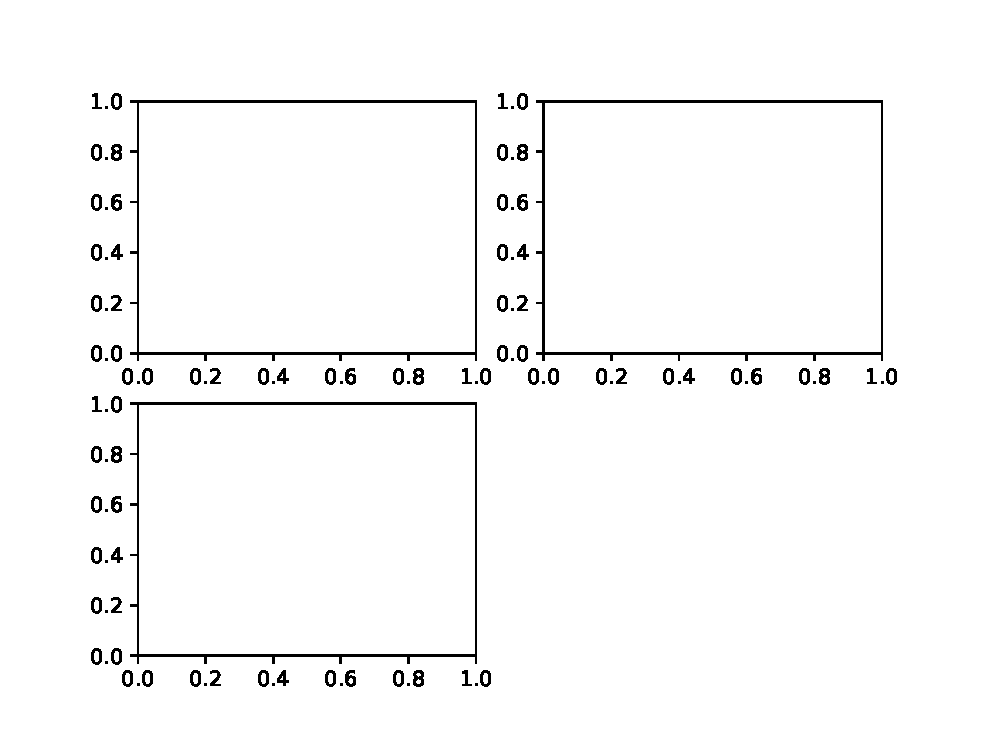
\includegraphics[width=10.0cm]{code/fig1.eps}
\vspace{-16pt}
\caption{\texttt{fig1.eps}}
\endframed
\end{center}
\end{figure}
%\begin{lstlisting}
%\end{lstlisting}
\end{cod}
\vspace{-20pt}

\subsection{2次元の散布図}

2次元の散布図は,\texttt{<axes>.scatter()}で描画することができる.散布図の場合は一つ一つの点がどれくらいの数値なのかがわかりにくいので,\texttt{<axes>.grid()}でグリッド補助線を追加する.また,各点についてどっちが$x$でどっちが$y$かわからないので横軸と縦軸に\texttt{<axes>.set\_xlabel(<str>)},\texttt{<axes>.set\_ylabel(<str>)}でラベルをつける.
\begin{gram} 
\begin{itemize}
\item \texttt{<axes>.scatter(x,y)}: 2次元データ$(\bm{x},\bm{y})$の散布図を描画する.ここで,$\bm{x},\bm{y}$は\texttt{<ndarray>}であり,左のデータが横軸,右のデータが縦軸である.
\item \texttt{<axes>.grid()}: \texttt{<axes>}にグリッド補助線を追加する.
\item \texttt{<axes>.set\_xlabel(<str>)}: \texttt{<axes>}の横軸にラベルをつける.
\item \texttt{<axes>.set\_ylabel(<str>)}: \texttt{<axes>}の縦軸にラベルをつける.
\end{itemize}
\end{gram}


\begin{rem}
基本的にmatplotlibに渡すデータは,\texttt{<ndarray>}であることが必要なので,以降はその前提とする.
\end{rem}

\begin{cod}[\texttt{fig2.py}] 
\lstinputlisting[backgroundcolor={\color[gray]{.95}}]{code/fig2.py}
\vspace{-19pt}
\begin{figure}[H]
\begin{center}
\framed
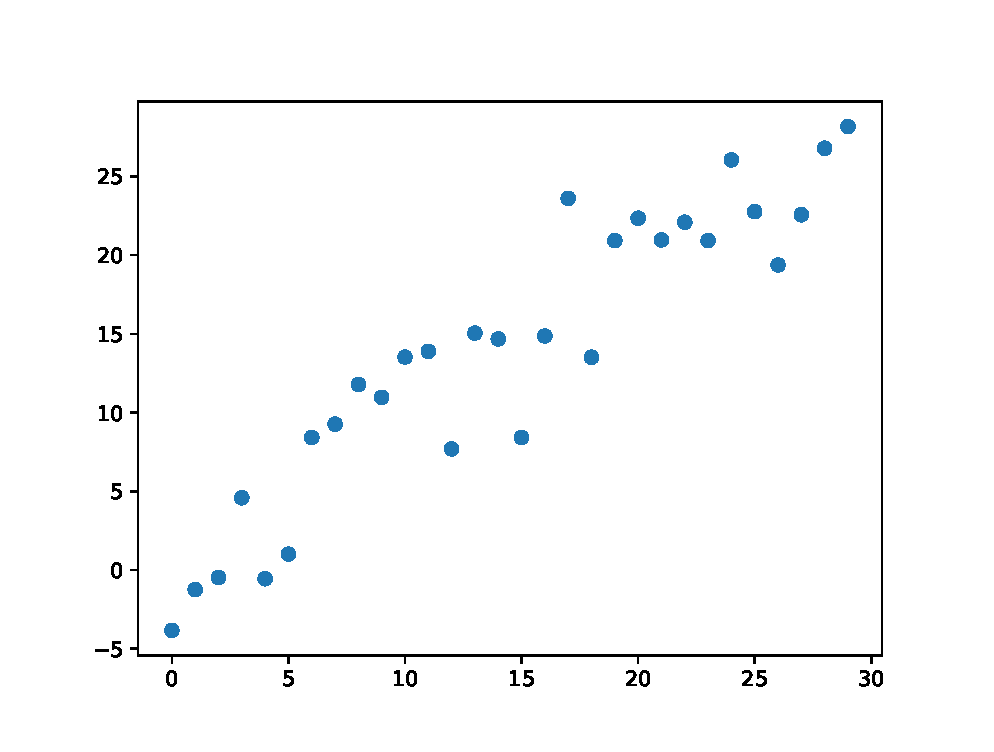
\includegraphics[width=8.0cm]{code/fig2.eps}
\vspace{-10pt}
\caption{\texttt{fig2.eps}}
\endframed
\end{center}
\end{figure}
%\begin{lstlisting}
%\end{lstlisting}
\end{cod}
\vspace{-20pt}